\documentclass[11pt,a4paper]{article}

%---------------------------------------------------------
%	Aditional Packages
%--------------------------------------------------------
\usepackage{textpos}
\usepackage{subcaption} % To have multiple plots side by side
\usepackage{float}
\usepackage{url} % enable clickable URLs
\usepackage{listings} % to have code blocks in your document
\usepackage{xcolor}
\usepackage{doi}
\usepackage{microtype}
\usepackage{booktabs}
\usepackage{nicefrac} % creates a fraction that is nicer when used in text \nicefrac{1}{2}

% Define some colors for code 
\definecolor{codegreen}{rgb}{0,0.6,0}
\definecolor{codegray}{rgb}{0.5,0.5,0.5}
\definecolor{codepurple}{rgb}{0.58,0,0.82}
\definecolor{backcolour}{rgb}{0.95,0.95,0.92}

% Defines codeblock styles
\lstdefinestyle{mystyle}{
    backgroundcolor=\color{backcolour},   
    commentstyle=\color{codegreen},
    keywordstyle=\color{magenta},
    numberstyle=\tiny\color{codegray},
    stringstyle=\color{codepurple},
    basicstyle=\ttfamily\footnotesize,
    breakatwhitespace=false,         
    breaklines=true,                 
    captionpos=b,                    
    keepspaces=true,                 
    numbers=left,                    
    numbersep=5pt,                  
    showspaces=false,                
    showstringspaces=false,
    showtabs=false,                  
    tabsize=2
}

% Set the maximum depth sections are counted to and shown in the TOC
\setcounter{secnumdepth}{3} % depth of counting
\setcounter{tocdepth}{3} % depth that toc will show 

% new paragraph style with new line
\newcommand{\myparagraph}[1]{\paragraph{#1}\mbox{}\\}


\lstset{style=mystyle}
\renewcommand{\lstlistingname}{Configuration}% Listing -> Configuration

% Toogle between the two to hide or show images
% \usepackage[draft]{graphicx}
\usepackage{graphicx}
\usepackage[utf8]{inputenc} 
\usepackage{upgreek}
\usepackage{titlesec}
\usepackage{physics} % adds easy derivatives etc. 
%\AtBeginDocument{\RenewCommandCopy\qty\SI} % dont know why
\usepackage{amssymb} % more symbols
\usepackage{amsmath} %enables align environment
\usepackage{multirow}


% \usepackage[showframe]{geometry} % Shows margins in pdf if you want to know what's going on
\usepackage{geometry}
\geometry{
    %a4paper,
	left=40mm,
    % right=20mm,
	top=35mm,
    }

% Use biblatex
\usepackage[backend=biber,
natbib=true,
maxcitenames = 2,
maxbibnames = 5,
minbibnames = 4, 
sorting=none]{biblatex}

\usepackage{csquotes}

\addbibresource{references.bib}
\setlength\bibitemsep{1.5\itemsep}


% --------------------------------------------------------
% CUSTOM STUFF:
\usepackage[textsize=tiny]{todonotes}
\setlength{\marginparwidth}{2cm}
\usepackage{bm}
%---------------------------------------------------------
\usepackage{hyperref} % enable clickable links to sections, figures, etc. 
\PassOptionsToPackage{unicode}{hyperref}
\PassOptionsToPackage{naturalnames}{hyperref}

% Remove the coloured border around autoref links
\hypersetup{%
pdfborder = {0 0 0}
}



\begin{document}	
\pagestyle{empty}

%---------------------------------------------------------
%	Titlepage
%---------------------------------------------------------

\begin{center}
    \vspace*{1cm}
    \LARGE \bf{Structure recognition with graph neural networks} \\

    \vspace*{2cm}
    \large \bf{An intermediate report for the course "Advanced Projects in Computational Physics 2"}


    \vspace{4cm}
    
    \vspace{1.2cm}
            From\\
            {\bf Stephen Weybrecht} \\
            \today

    \vspace*{6 cm}
    Supervisor: Jonas Buba 
    \vspace*{1 cm}

\end{center}
\clearpage

\begin{abstract}
    The project described in the following lies at the intersection of solid state physics and machine learning. On the one hand there is the physical problem, namely the classification of noisy crystal lattices in 2 and 3 dimensions into their corresponding Bravais lattice group. For this graphs are randomly generated in a first step. These graphs then need to be classified efficiently and robustly, regardless of noise and introduced defects. As is the case with other classification tasks, neural networks promise an interesting approach to this goal and will therefore be the second part of this project. For this special networks designed for handling graph like structures, so called Graph convolutional networks are employed. These use a concept called message passing to efficiently enable graph level classification tasks. \\
    
    By use of these concepts a test accuracy of over 90\% has been achieved for both the 2D and 3D case. Future goals include testing out other features and network architectures for this classification task, as well as the specialisation in defect detection in mono atomic crystal lattices.

    
\end{abstract}
%---------------------------------------------------------
%	Table of Contents
%---------------------------------------------------------
% Generate
\newgeometry{
    %a4paper,
	%left=20mm,
    right=40mm,
	top=35mm,
    } 
\tableofcontents
\restoregeometry
\clearpage
\mbox{}

\pagenumbering{arabic}
\setcounter{page}{1}
 \pagestyle{plain}
%---------------------------------------------------------
%	Report
%---------------------------------------------------------

\section{Theoretical introduction}
\label{sec:Theoretical introduction}

\subsection{Bravais lattices}
\label{ssec:Bravais lattices}
In the first part of the project, our task was to deal with crystal lattices in 2 and 3 dimensions. 
For the following discussion an introduction of the terms "crystal", "basis" and "Bravais lattice" is therefore needed. \\

Following the discussion of \cite{kittelChapter1Crystal2005} an ideal crystal is a periodic, infinite arrangement of atoms in a solid. 
These atoms are arranged in blocks, a so called basis, in a regularly spaced grid, the lattice. 
In other words the lattice represents a schema after which individual atoms or groups of atoms (the basis) are arranged to form the crystal. 
A lattice in $d$ dimensions can be defined by a set of $d$ translation vectors. 
The superposition of integer multiples of these vectors then makes up the lattice \cite{kittelChapter1Crystal2005}. 
In principle the length and direction of these vectors can be arbitrary. 
In this case the lattice would generally not map into itself under translations and rotations -- the lattice is called oblique. 
There are however special sets of translation vectors which form lattices of high symmetry. 
These fundamental lattices are called the Bravais lattices. 
For $d=2$ there are 5 (4 special and one oblique) Bravais lattices, while for $d=3$ there are 14 (13 special cases and one oblique, so called triclinic lattice). 
These are depicted in \autoref{fig:bravais2D} and \autoref{fig:bravais3D} respectively. 

\begin{figure}[htbp]
    \centering
    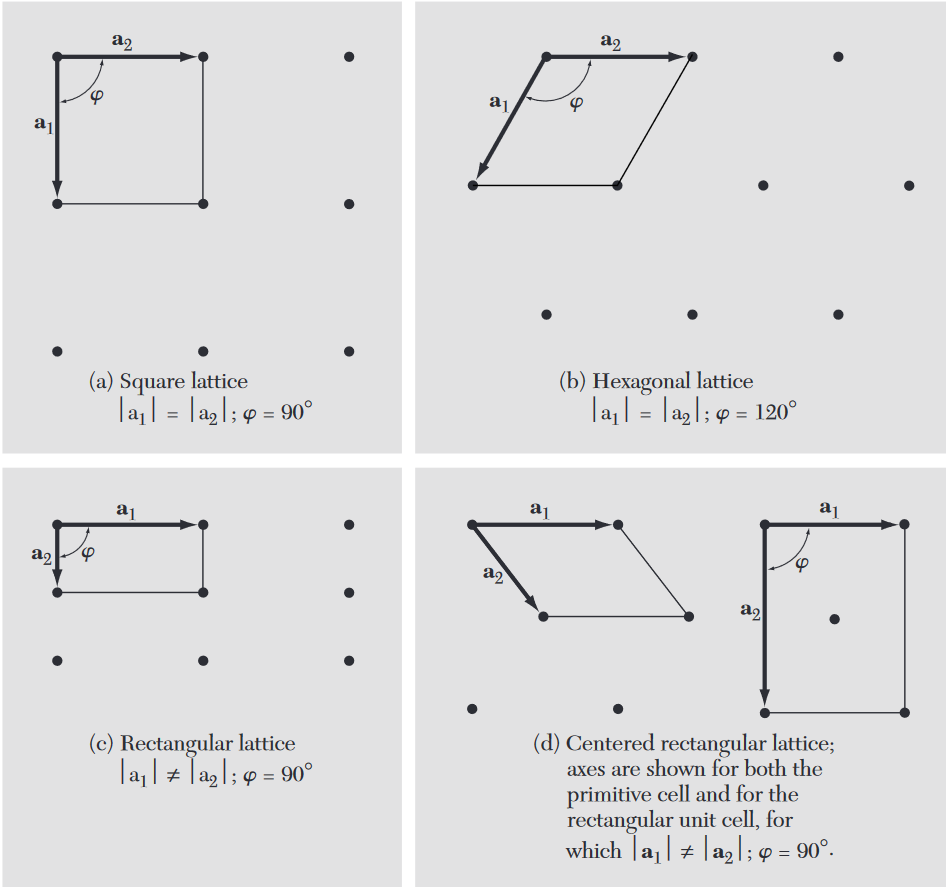
\includegraphics[width=0.6\textwidth]{images/Kittel_7.png}
    \caption{The five Bravais lattices for 2 dimensions. The graphic also illustrates the length of the translation vectors $\bm{a}_i$ and the angle between them in order to make up the corresponding lattice. Taken from \cite[Fig. 7]{kittelChapter1Crystal2005}.}
    \label{fig:bravais2D}
\end{figure}

\begin{figure}[htbp]
    \centering
    \includegraphics[width=0.7\textwidth]{images/Kittel_14.png}
    \caption{The 14 Bravais lattices for the $d=3$ case. 
    One further classifies these lattices into seven types of cells: Cubic ($a{=}b{=}c$, $\alpha {=} \beta {=} \gamma{=}90^\circ$), Tetragonal ($a{=}b {\neq} c$, $\alpha {=} \beta {=} \gamma{=}90^\circ$), Orthorhombic ($\alpha {=} \beta {=} \gamma{=} 90^\circ$), Monoclinic ($\alpha {=} \beta{=}90^\circ {\neq} \gamma$), Triclinic, Triagonal ($a{=}b{=}c$, $\alpha {=} \beta {=} \gamma <120^\circ {\neq} 90^\circ$), Hexagonal ($a{=}b{\neq} c$, $\alpha {=} \beta{=} 90^\circ, \gamma{=} 120^\circ$). 
    Note that in the prior notation $a$, $b$ and $c$ denote the lengths of the translation vectors, $\alpha$, $\beta$, $\gamma$ the angles between them and omitted length or angle relations mean they can be arbitrary. 
    These groups are again subclassified based on their lattice structure into simple "P", body-centred "I", base-centred "C", face-centred "F". 
    As mentioned, all lattices are special cases of the general, triclinic case. The graphic is taken from \cite[Fig. 14]{kittelChapter1Crystal1971}.}
    \label{fig:bravais3D}
\end{figure}


\subsection{Basics of Machine Learning}
\label{ssec:BAsics of Machine Learning}
In the following the basic principles behind Artificial Neural Networks (NNs) and Machine Learning will be explained. 
This chapter follows closely the discussion in \cite{kubatChapter5Artificial2017}, the upcoming equations and concepts are therefore taken from this source. 
For this introduction the simplest model will be used as an example to explain the key concepts, as a generalisation to more sophisticated models is straightforward once the basic principles are understood. 
This simple model is the so called Perceptron, a network consisting of fully connected units, so called neurons, aranged in layers. 
This NN consists at least of an in- and output layer which are usually supplemented by one or more hidden layers in between. 
A neuron $j$ in layer $l$ has as its attribute a feature vector $x^{(l)}_j$ and each connection is associated by a weight $w_{ij}^{(l-1)}$ where this weight represents the connection between neuron $i$ in layer $l-1$ to neuron $j$ in layer $l$. 
The general idea is that each neuron takes as input the "signals" from every neuron it is connected to in the previous layer (ie. in our example of a fully connected network the signals from every neuron in the prior layer) and updates its own value according to the fololowing weighted sum:
\begin{equation}
    \label{eq:NN weighted sum}
    x^{(l)}_j = f\left(\sum_i w_{ij}^{(l-1)} \cdot x^{(l-1)}_i + b^{(l-1)}\right)
\end{equation}
Here the weighted sum is further modified by a layer dependent bias vector $ b^{(l-1)}$. 
Furthermore the aggregated "signal" is usually modified by an non-linear activation function $f$. 
Using the above update rule it is now clear, that a forward pass through the model can be accomplished by suppliing an input vector $x^{(1)}_i$ and using \autoref{eq:NN weighted sum} iteratively to achieve an output at the final layer $n$ $x^{(n)}_i$. \\

In this simple supervised training example each input vector $x^{(1)}_i$ is acommpined by a target vector $t_i$ which is the wanted output of the network, given said input vector. 
For training one must now specify a so called loss function, which represents how far the output of the NN deviates from said target (e.g. the mean squared difference between them). 
It is apparent that the goal of training must be to minimize said loss. 
This is done via so called gradient descent where the gradients of the loss function with respect to the model parameters $w_{ij}^{(l-1)}$ and  $ b^{(l-1)}$ is calculated. 
In the parameter space of these weights and biasses this gradient points toward regions where the loss changes the most. 
In the process of backpropagation the NN parameters are now updated using these gradients. 
The algorithm goes backwards through the network (From layer $n$ to $1$) and updates the paramaters using calculated gradients such that the loss is minimized. 
The magnitude of this update is influenced by the Learning rate $\eta$ which is an important hyperparameter that needs to be set for training. 
How this update works in detail goes beyond the scope of this introduction, further details can for example be found in \cite{kubatChapter5Artificial2017}. 
Once this training is completed for all input training samples one epoch of training has been completed. 
Usually the training of a NN is repeated for many epochs. \\

Lastly, once the training was deemed sufficient, one used a different, so called validation dataset, which was not used during training to asess the final performance metric of the model. 

\subsection{Graph neural networks}
\label{ssec:Graph neural networks}
The lattices as discussed in the prior section are a collection of atoms linked by bonds and can therefore be suitably represented by a graph, consisting of nodes and edges. 
If we want to apply machine learning to crystal lattices, we therefore need models that are well suited for data organized in a graph-like manner. 
What follows is a basic introduction to such networks, specifically graph convolutional neural networks (GCNs). \\

GCNs take inspiration in the already well-established convolutional neural networks in which a typical layer consists of a trainable kernel that can be applied on ordered, grid-like training data of arbitrary size and shape (e.g.. images) \cite{khemaniReviewGraphNeural2024}. 
GCNs represent a generalisation of this concept onto unordered nodes with a variable number of neighbours. 
Each GCN-layer uses so called message passing in order to update the node state $h^{(t)}_u$ of a time $t$ to the next step $h^{(t+1)}_u$ as shown in \autoref{eq:messagepassing} \cite[eq. 4.1]{khemaniReviewGraphNeural2024}.
\begin{equation}
    h^{(t+1)}_u = UPDATE^{(t)}\left(h^{(t)}_u, AGGREGATE^{(t)}\left(\left\{h^{(t)}_v, \forall v \in N(u)\right\}\right)\right)
    \label{eq:messagepassing}
\end{equation}
In the above equation $UPDATE^{(t)}$ and $AGGREGATE^{(t)}$ could be any differentiable functions i.e. also neural networks, and $N(u)$ denotes the neighbourhood of $u$ meaning all directly connected nodes in the graph. 
This equation implies the following update schema that is also depicted in \autoref{fig:messagepasisng}: \\
The starting point is a graph, consisting of nodes with feature vectors and connections, that could also have features. 
For each node, messages from neighbouring nodes are aggregated to a single message by taking a weighted mean of the neighbouring nodes feature vectors. 
This operation can also be weighted by use of edge features. 
This message is then passed to a non-linear update function (e.g.. ReLU), that updates the node in question for the next time step. 
After the update is completed, further operations can be performed depending on the wanted classification scheme. 
In the following graph classification is used, which means all feature vectors are pooled in a last step, in order to get a single quantity that is descriptive of the entire graph \cite{khemaniReviewGraphNeural2024}.
\begin{figure}[htbp]
    \centering
    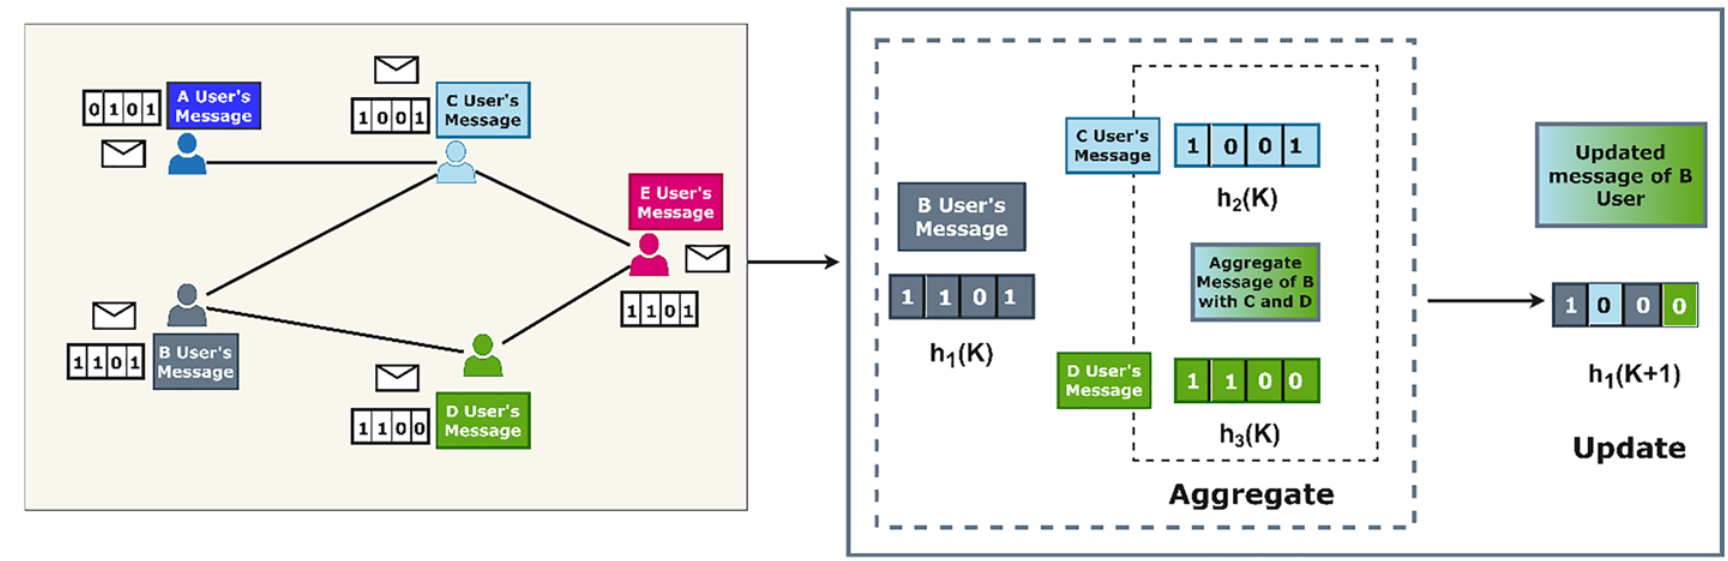
\includegraphics[width=0.9\textwidth]{images/khemani7.png}
    \caption{A graphic representation of the update schema for message passing graph neural networks. Taken from \cite[Fig. 7]{khemaniReviewGraphNeural2024}.}
    \label{fig:messagepasisng}
\end{figure}

\todo{SSec (graph) autoencoders}

\section{Results}
\label{sec:Results}
In the following I will give a chronological overview of the topics I worked on during this project. 
This started with the generation of training data, namely Bravais lattices in two and three dimesions. After this I worked on Bravais lattice classification of noisy and defective lattices to gain familiarity with the GNN architecture and a Machine Learning library. Lastly I worked on defect detection using Graph Autoencoders. 

\subsection{Generation of Training data}
\label{ssec:Generation of training data}
As a first step Bravais lattices in two dimensions (2D) and three dimensions (3D) needed to be created. 
For this ideal Bravais lattices with roughly a unit spacing between nodes are created in a first step. 
Additionally random Gaussian noise is added. 
For further variety in training samples, graphs are additionally scaled by random constants to provide non-uniform node-spacing within one Bravais lattice group. 
At this step different kids of defects are introduced. 
These defects either are a removal of randomly many nodes at random positions or the addition of a single, randomly placed node within the lattice. 
What kind of process has been used will be explained in detail in the following sections, as it is dependent on the task at hand. 
After the nodes have been placed, noise was added and defects were introduced, the connections between nodes are determined by searching for the neighbours within a given radius (that also depends on the noise amplitude) and connecting all nodes, that lie within said radius. 
By these means the random noise and defects are also included within the structure of the graph and have an influence in message passing. \\

The features used depend on the task of the GNN -- either graph classification into one of the Bravais lattice groups or defect detection. 
In the following a in-depth overview over all different features used is given such that the later sections can focus on the Neural Network part. \\
As edge features a selection of the following was used: 
\begin{itemize}
    \item The 2D or 3D connection vectors between nodes
    \item Their respective length
\end{itemize}
The node features tested are the following:
\begin{itemize}
    \item The amount of nearest neighbors i.e. the count of connected nodes
    \item The bond orientational order parameter (BOO)\\
    As the name suggests the BOO quantifies the "order" of the bonds around a node. 
    It can be computed for different orders $l$ and can be used to differenciate between different crystal sructures by quantifying their $l$-fold symmetry, see e.g. \cite{steinhardtBondorientationalOrderLiquids1983}. 
    Importantly symmetry is broken near defects, which is why the BOO seems a promising node feature for defect detection. 
    In 2D the BOO of node $j$ and order $l$ is given by
    \begin{equation}
        \mathrm{BOO^{2D}}_j = \left|\frac{1}{N} \sum_k \mathrm{exp}(il\theta_{jk}) \right|^2
    \end{equation}
    Where we sum over all $N$ neighbors $k$ of node $j$ and $\theta_{jk}$ represents the angle of the $j$-$k$-connection with resprect to some reference direction. \\
    In 3D I used was one of the rotational invariants defined as 
    \begin{equation}
        \mathrm{BOO^{3D}}_j = \sqrt{\frac{4\pi}{2l+1} \sum_{m=-l}^{l} \left| \frac{1}{N} \sum_k Y_{lm}\right|^2}
    \end{equation} 
    Here the sum ranges again over all neighbors $k$ and adds the spherical harmonics $Y_{lm}$ dependent on the given order of the BOO and the angles between nodes $j$ and $k$ and an arbitrary refrence direction. 
    \todo{CITATIONS}
    As symmetry is also broken at the edges of the generated graphs, for the calculation I take care to apply sufficient padding of extra nodes around the graph (which are later removed) in order to mitigate edge effects. 
\end{itemize}


\section{Results so far}
\label{sec:Results so far}
\todo{ Wie groß war der Datensatz? Wie wurde er aufgeteilt für
Training/Validation}
\todo{Wie lief der Trainingsprozess ab? (Optimizer, batchsize, learning
rate etc., gerne loss/accuracy plotten)}
\todo{ * Verwendete Layer und Aufbau des Netzes beschreiben (welche Methode
wurde für das Pooling verwendet? wie kommen wir vom Pooling zu
unserer Wahrscheinlichkeitsverteilung der Gittertypen?)}
The main tasks so far were to gain familiarity with a machine learning Python library by working on graph classification of 2- and 3-dimensional Bravais lattices. 
For this I chose PyTorch, as it has a library for working with graph neural networks called PyTorch Geometric (PyG) built on top of it. 
The first step for both cases was to generate the training data. 
For this ideal Bravais lattices were created in a first step, to which random (Gaussian) noise, and defects (meaning a removal of a random number of nodes at random positions) were added. 
For further variety in training samples, graphs were additionally scaled by random constants to provide non-uniform node-spacing within one Bravais lattice group. 
After the nodes have been placed and noise was added, the connections between nodes are determined by searching for the neighbours within a given radius (that also depends on the noise amplitude) and connecting all nodes, that lie within said radius. 
By these means the random noise and defects are also included within the structure of the graph and have an influence in message passing. \\
The size of the graphs have been chosen as follows. 
For the plane lattices a size of 10 by 10 nodes has been chosen in order to give the network enough information about each training sample to learn something about the Bravais lattice. 
For the 3D lattices a  size of 10 by 10 by 10 nodes has been tried but deemed unpractical as the time effort for training is quite large. 
This in turn leads to only being able to use a low number of training samples which leads to low accuracies of around 60\%. 
A better approach proved to be using graphs of size 5 by 5 by 5 nodes which cuts the total number of nodes per graph by a factor of 8 while still giving the network enough information to determine the lattice correctly. \\
For node features the number of neighbouring nodes has been chosen while each edge has the (two or three dimensional) connection vector between its corresponding nodes as its feature. 
This has proven itself to be enough information to classify a test dataset of random graphs with more than 90\% accuracy for both cases. 
For classification each lattice was labeled by its one-hot encoded type that was then compared by using the  cross entropy loss function during training. 
As connection vectors carry quite a lot of information, for future tests other features like connection lengths or binding angles are planned in order to see, how much information about the lattice is needed to suitably classify it. 
For these preliminary results a high degree of information in the features and shallow neural network (2D: 2 GINEConv layers \cite{pygteamGINEConv2024} with a total of 12 hidden neurons, 3D 3 GINEConv layers with 50 hidden neurons total) was however used as a proof of concept and to see whether graph generation worked. 



\section{Plans for the future}
\label{sec:Plans for the future}
In the following the goals for the remaining part of the project will be discussed and a rough time estimate for each step will be given. 
As graph generation and classification has worked rather well so far, I expect only little changes to be made to the already existing code. 
Further things to improve or try out with the existing method are varying node and edge features and choosing different layers or a different network structure. 
By this investigation one could find out the minimal amount of information the network needs to classify Bravais lattices and the most efficient network architecture. 
As the tasks discussed so far however only served as a kind of general introduction into the actual topic that is specific to me, extensive experiments with the old goal of lattice classification are not planned. 
Instead the focus shifts towards a new goal, namely the detection of defects in mono atomic crystals. 
I expect to be able to reuse significant parts of the lattice generation code I have written so far, although significant changes in the network architecture and features will most likely be made. 
A meeting with Jonas Buba for discussing the specifics for the future project is scheduled for Wednesday, the 11.12. 
After that I plan to finish the remaining experiments having to do with the old goal of Bravais lattice classification until the end of December. 
During the same time I want to gain familiarity with the theory and suitable approaches for defect detection by reading literature and starting to code. 
Until the mid of January I plan to finalise the coding part of the project, to be able to focus on writing the report and preparing the final presentation during the remaining time. 

\section{Code availability}
\label{sec:Code availability}
The code written for this project is made available in the following Git repository: \url{https://github.com/SteWey0/Computerpraktikum/}

%---------------------------------------------------------
%	Bibliography
%---------------------------------------------------------

\newgeometry{
	%a4paper,
	left=40mm,
    % right=20mm,
	top=35mm,
}
\renewcommand\refname{Bibliography}
% \printbibliography
\printbibliography[
heading=bibintoc,
title={Bibliography}
]


\end{document}